%!TEX root=thesis.tex
\chapter{Galaxies and Active Galactic Nuclei}
\label{cha:astro}

    Modern astronomy relies on observations of deep space. Telescopes image the sky in different wavelengths, with different wavelengths carrying different physical meanings. Infrared surveys detect star formation and dust in distant galaxies, and radio surveys detect massive objects called active galactic nuclei. In this section, I introduce the physics of what we see when we look at the sky in these wavelengths, as well as introducing specific radio and infrared surveys relevant to this thesis. I will also discuss the motivation behind cross-identifying active galactic nuclei with their host galaxies as well as the inherent difficulty in doing so, and hence the motivation behind this thesis.

    % \section{Galaxies}

    % \section{Supermassive Black Holes and Active Galactic Nuclei}

        % Black holes are compact, dense objects of extraordinarily large mass. Due to their density, black holes have extremely strong gravitational fields, and any object that gets close enough will be unable to escape \citep{wald10}. This even includes light, which is effectively absorbed by black holes, giving them their name.

        % \todo{Talk about how black holes are predicted by GR.}

        %     More information on black holes and general relativity can be found in \citet{wald10}.

        % \todo{Talk about how we can observe black holes?}

    \section{Active Galactic Nuclei}

        Many galaxies contain a supermassive black hole in their centre. These black holes accrete matter from the surrounding galaxy in an accretion disk \todo{figure}. The accretion process emits huge amounts of light through different physical processes. These light-emitting black holes are called active galactic nuclei (AGNs). AGNs can be extremely bright, emitting up to $10^{39}$ J of energy every second --- nearly a thousand times more energy than our entire galaxy emits \citep{begelman84}. AGNs are found throughout the universe: The closest known AGN is Centaurus A (shown in Figure \ref{fig:centaurus-a}, with $z \approx 0.0018$, and AGNs have been detected up to redshifts of $z \approx 7$ \todo{citation needed}.

        \begin{figure}[!ht]
            \centering
            \includegraphics[width=0.5\textwidth]{images/ESO_Centaurus_A_LABOCA.jpg}
            \caption{Centaurus A, a relatively close radio active galactic nuclei. \emph{Image: ESO/WFI (Optical); MPIfR/ESO/APEX/A.Weiss et al. (Submillimetre); NASA/CXC/CfA/R.Kraft et al. (X-ray)}}
            \label{fig:centaurus-a}
        \end{figure}

        Many AGNs produce \emph{jets} from their accretion disk. Jets are long, thin streams of matter such as the one shown in Figure \ref{fig:m87}. These jets can be very long, with ``giant'' AGNs emitting jets up to 1 Mpc in length \todo{citation needed --- maybe \citet{banfield16}?}. The process through which jets are emitted is currently unknown \todo{citation needed}.
        %--- for example, the jet in Figure \ref{fig:m87} is $1.5$ kpc in length \citep{rees87}.

        \begin{figure}[!ht]
            \centering
            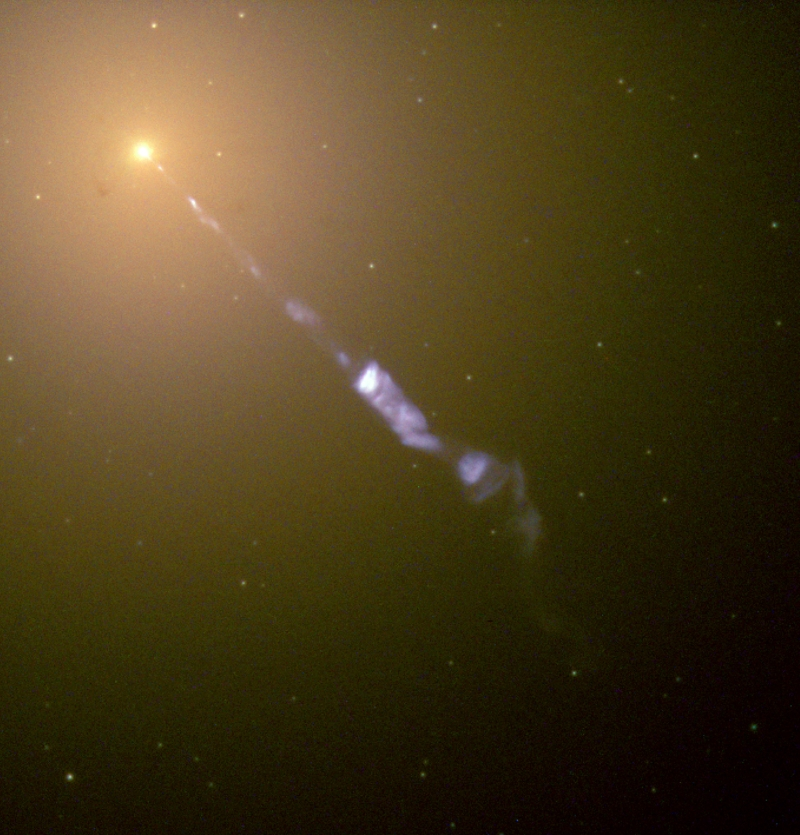
\includegraphics[width=0.5\textwidth]{images/M87_jet.jpg}
            \caption{M87, a giant elliptical galaxy with a jet. \emph{Image: NASA and The Hubble Heritage Team (STScI/AURA)}}
            \label{fig:m87}
        \end{figure}

        Electrons in jets produce \emph{synchrotron radiation}, a form of radiation emitted by charged particles as they accelerate at relativistic speeds in a magnetic field \todo{citation needed}. This radiation is emitted in radio wavelengths, and so AGNs emitting this kind of radiation are called \emph{radio AGNs}. It is radio AGNs that are the focus of this thesis, and from this point on, ``AGN'' will refer only to radio AGNs.

        While we cannot observe the black holes of AGNs directly, we can observe the radio emissions from their jets. \todo{Keep motivating! Read those articles Julie suggested.}

        % \begin{figure}[!ht]
        %     \centering
        %     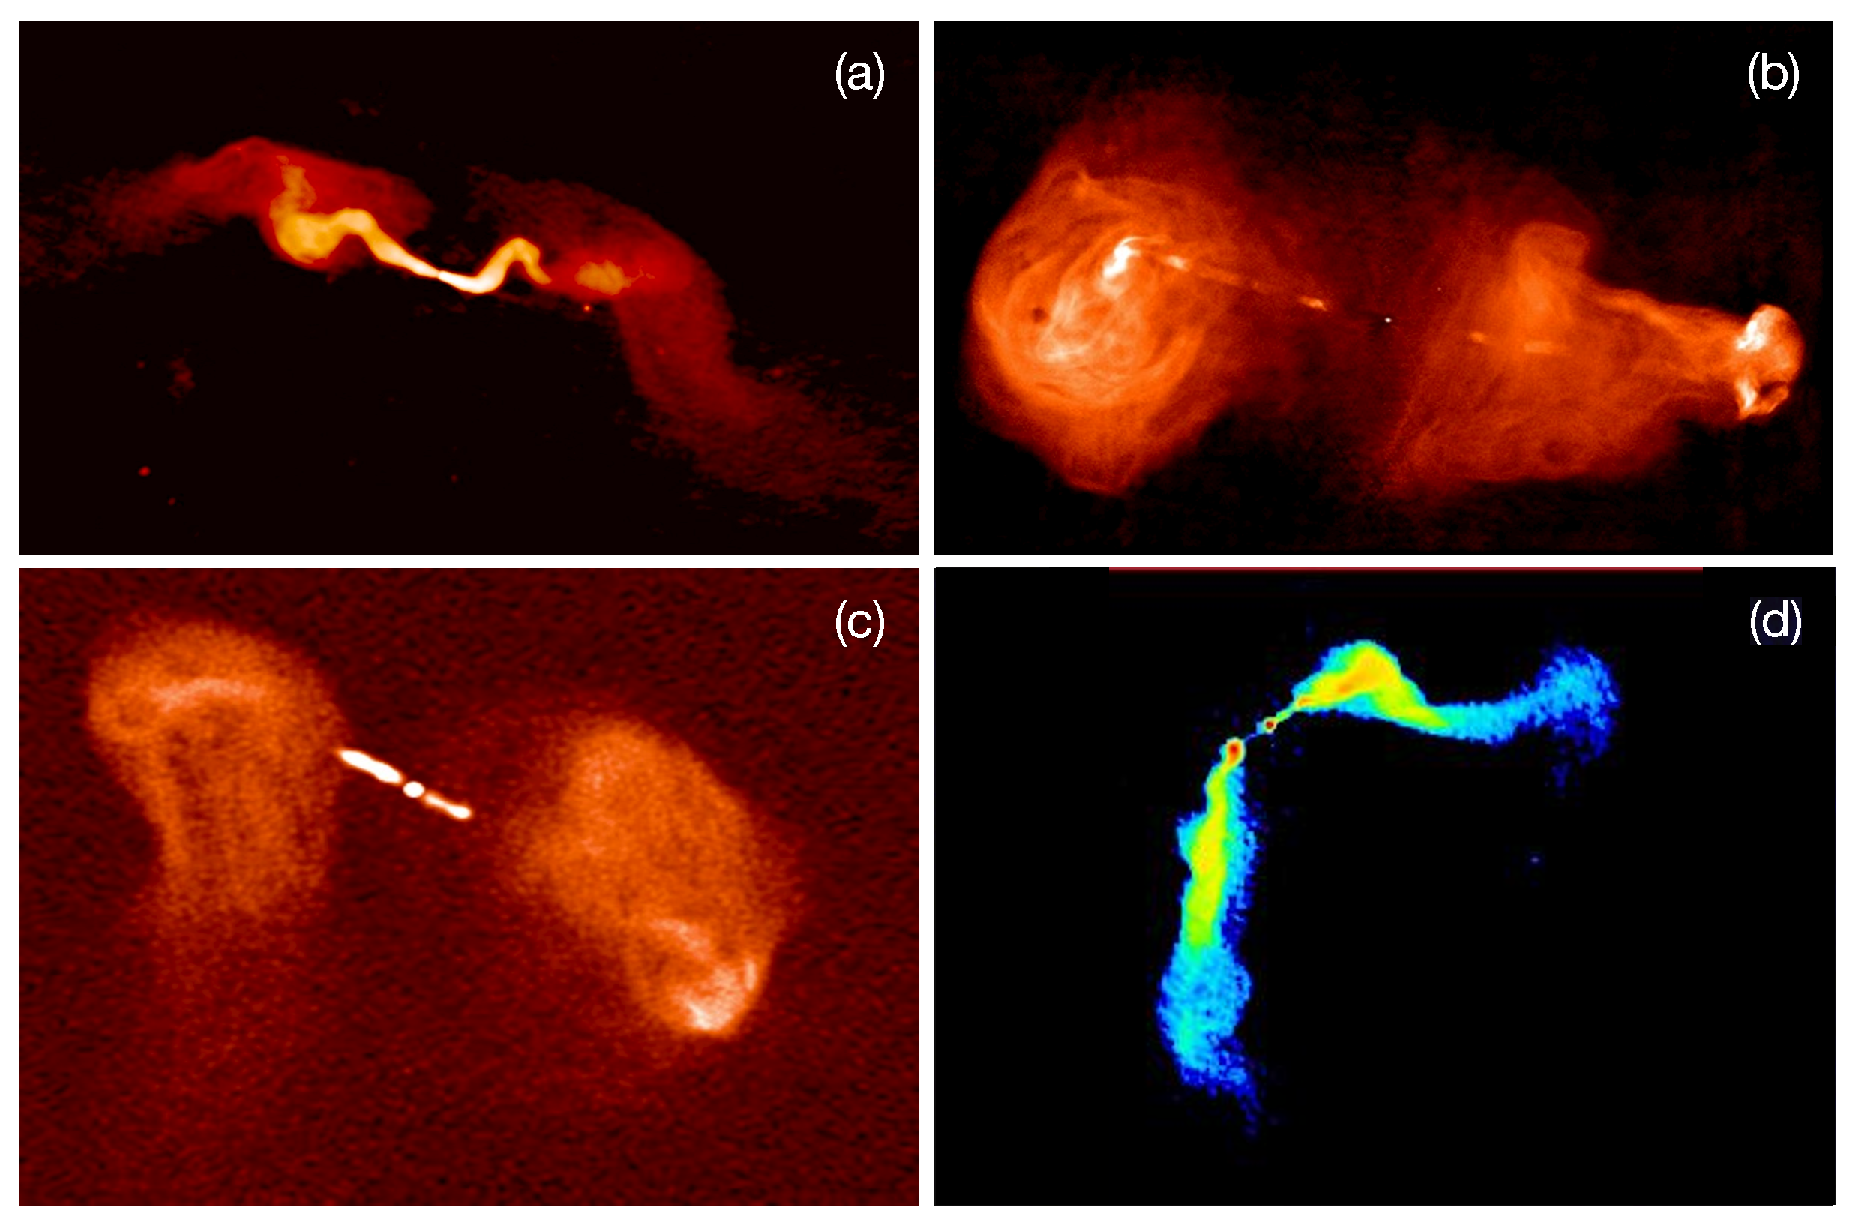
\includegraphics[width=0.8\textwidth]{images/rgz_fig1.eps}
        %     \caption{Different shaped radio AGNs. Figure reproduced from \citet{banfield15}.}
        %     \label{fig:radio-agns}
        % \end{figure}

    \section{Astronomical Observations}

        When observing the sky, we can think about the sky as a spherical surface surrounding the earth. All objects we see with telescopes are flat on the sky, and we only have limited tools to determine their distances and scales. In this section, I will describe the coordinate systems used to describe these objects, and outline some of the challenges associated with astronomical observations.

        \subsection{Astronomical Coordinates}

            Astronomy uses a coordinate system called the \emph{equatorial coordinate system} to describe the positions of objects on the sky. Each position on the sky is described by two numbers: the \emph{right ascension} (RA) and the \emph{declination} (dec).

            \begin{figure}[!ht]
                \centering
                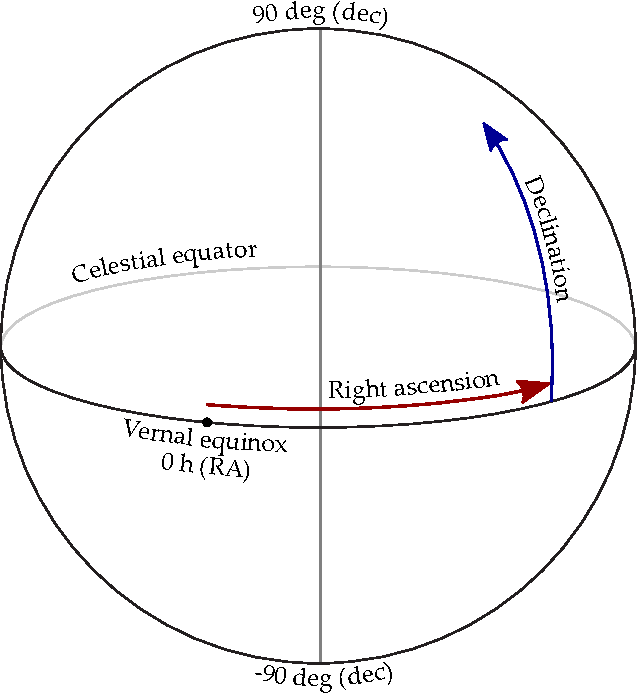
\includegraphics[width=0.5\textwidth]{images/ra-dec}
                \caption{The equatorial coordinate system.}
                \label{fig:equatorial-coordinates}
            \end{figure}

            The right ascension of an object is the angle eastward from the vernal equinox to the object along the celestial equator. It is measured in hours (h), minutes (min), and seconds (s). There are 60 seconds in 1 minute, 60 minutes in 1 hour, and 1 hour is equal to 15 degrees. Right ascension ranges between 0h and 24h, where both 0h and 24h are located at the vernal equinox. The declination of an object is the angle northward from the celestial equator to the object. It is measured in degrees (${}^\circ$), arcminutes ($'$), and arcseconds ($"$). Declination ranges between $-90^\circ$ and $90^\circ$, where $-90^\circ$ is the declination of the south celestial pole and $90^\circ$ is the declination of the north celestial pole. The right ascension and declination are shown in Figure \ref{fig:equatorial-coordinates}. It is important to note that while right ascension and declination are both measured in minutes and seconds, these are \emph{different} minutes and seconds. 1 minute (right ascension) is equal to 15 arcminutes (declination).

            Objects are usually given a International Astronomical Union (IAU) name based on their coordinates. This name includes the catalogue that identified the object, the right ascension, and the declination. For example, ATLAS3 J002925.7-440256C is from the third release of the ATLAS catalogue, and is located at 00h 29m 25.7s $-44^\circ$ $02'$ $56"$.

            \todo{Write about epochs.}

        \subsection{Redshift}

    \section{ATLAS: The Australia Telescope Large Area Survey}

        \begin{figure}[!ht]
          % \centering
          \includegraphics[width=0.8\linewidth,]{images/CDFS_sm.eps}
          \caption{ATLAS observations of CDFS. Reproduced from \citet{franzen15}.}.
          \label{fig:cdfs}
        \end{figure}

        The Australia Telescope Large Area Survey (ATLAS) is a deep \todo{define?} survey of two small areas of the sky in radio wavelengths, which aims to help understand the evolution of early galaxies \citep{norris06}. The Australia Telescope Compact Array was used to image the Chandra Deep Field South (CDFS) and the European Large Area ISO Survey - South 1 (ELAIS-S1) fields. These fields are areas of the sky with few nearby objects, meaning that observations in these fields are of very old, distant objects. These fields were chosen because they are the two fields imaged in the Spitzer Wide-area Infrared Extragalactic Survey (SWIRE) visible from the southern hemisphere. SWIRE produced high-resolution infrared and optical images of the fields, allowing all objects detected in the ATLAS radio images to be compared with their infrared and optical counterparts.

        ATLAS is considered a pilot survey for the Evolutionary Map of the Universe (EMU), an upcoming radio survey of the entire southern sky at resolutions 45 times higher and angular resolutions 4.5 times better than the benchmark NRAO VLA Sky Survey \citep{norris11b}. EMU will use the new Australian Square Kilometre Array Pathfinder (ASKAP) telescope to image the same radio frequencies as ATLAS at the same resolutions, so tools and methods developed to process and interpret ATLAS data are expected to work well on the data produced by EMU. While ATLAS covers a total area of 6.4 deg$^2$, EMU will cover $75\%$ of the sky \citep{norris11b, norris16}. EMU is expected to detect around 70 million radio objects, compared to the 2.5 million currently known \citep{banfield15}.

        ATLAS provides both a catalogue of detected radio objects and a radio image of the CDFS and ELAIS-S1 fields. The CDFS image covers a total area of 3.7 deg$^2$ and the ELAIS-S1 image covers a total area of 2.7 deg$^2$. The CDFS image is shown in Figure \ref{fig:cdfs}. The catalogue is a list of all objects detected in the images with a peak or integrated flux more than 5 times the background noise levels. Each object has an associated survey identifier, an IAU name, a position on the sky of the peak flux, a peak flux density, an integrated flux density, an angular size, whether the object is extended or compact, and a spectral index, as well as uncertainties associated with each measurement \citep{franzen15}.

    % \section{Infrared Surveys}

    %     \subsection{WISE}

    % \subsection{SWIRE}

    % \section{Radio Surveys}

    %     \subsection{FIRST}

    %     \subsection{ATLAS}